% !TeX root = ../main.tex

\section{Free electron model}

\begin{problem}
  Two-charge-carrier Drude model:

  Consider a system of two types of charge carriers in the Drude model.
  The two carriers have the same density ($n$)
  and opposite charge ($e$ and $-e$),
  and their massesand relaxation rates are $m_1$, $m_2$ and $\tau_1$, $\tau_2$,
  respectively.
  So their corresponding mobilities are $\mu_1 = \frac{e\tau_1}{m_1}$ and
  $\mu_2 = \frac{e\tau_2}{m_2}$, respectively.
  \begin{enumext}[label = (\alph*)]
    \item Calculate the magnetoresistance $\Delta \rho = \rho(B) - \rho(B = 0)$,
    where $B$ is the magnetic field.
    \item Calculate the Hall coefficient.
    \item In an undoped semiconductor, $n = n_0 \upe^{-\Delta/k_BT}$
    describes the temperature dependence of the carrier concentration.
    What will the temperature dependence of the magnetoresistance
    and the Hall coefficient be?
  \end{enumext}
\end{problem}
\begin{solution}\leavevmode
  \begin{enumext}[label = (\alph*)]
    \item For the two carriers, we have
    \[
      \sigma_{0i} = \frac{ne^2\tau_i}{m_i} = ne\mu_i,\quad
      \omega_{ci} = \frac{eB}{m_i},\quad
      \omega_{ci}\tau_i = \mu_iB
    \]
    The total conductivity tensor is
    \[
      \hat\sigma = \hat\sigma_1 + \hat\sigma_2
    \]
    and the components are
    \begin{align*}
      \sigma_{xx} & = \frac{ne\mu_1}{1 + (\mu_1B)^2}
                    + \frac{ne\mu_2}{1 + (\mu_2B)^2}\\
      \sigma_{xy} & = \frac{ne\mu_1^2B}{1 + (\mu_1B)^2}
                    + \frac{ne\mu_2^2B}{1 + (\mu_2B)^2}\\
      \sigma_{zz} & = ne(\mu_1 + \mu_2)
    \end{align*}
    The resistance tensor is the inverse
    \[
      \hat\rho = \hat\sigma^{-1}
    = \frac{1}{\sigma_{xx}^2 + \sigma_{xy}^2}
    \begin{pmatrix}
      \sigma_{xx} & -\sigma_{xy} & 0\\
      \sigma_{xy} & \sigma_{xx}  & 0\\
      0 & 0 & \frac{\sigma_{xx}^2+\sigma_{xy}^2}{\sigma_{zz}}
    \end{pmatrix}.
    \]
    Then, the element $\rho_{xx}$ becomesrt
    \[
      \rho_{xx}(0) = \sigma_{xx}^{-1}(0) = \frac{1}{ne(\mu_1 + \mu_2)}, \qq{and}
      \rho_{xx} = \frac{\sigma_{xx}(B)}{\sigma_{xx}^2(B) + \sigma_{xy}^2(B)}
    \]
    So, the magnetoresistance is
    \[
      \Delta \rho = \rho_{xx}(B) - \rho_{xx}(0)
    = \frac1{ne}\ab[
      \frac{\frac{\mu_1}{1+(\mu_1B)^2} + \frac{\mu_2}{1+(\mu_2B)^2}}
        {\ab(\frac{\mu_1}{1+(\mu_1B)^2} + \frac{\mu_2}{1+(\mu_2B)^2})^2
    + B^2\ab(\frac{\mu_1}{1+(\mu_1B)^2} - \frac{\mu_2}{1+(\mu_2B)^2})^2} -
      \frac1{\mu_1 + \mu_2}]
    \]
    \newpage
    \item Since
    \[
      \rho_{xy}(B) = -\frac{\sigma_{xy}(B)}
        {\sigma_{xx}(B)^2 + \sigma_{xy}(B)^2},
    \]
    subsitute it into the definition of Hall coefficient
    $R_H = \frac{\rho_{xy}}{B}$, that is
    \[
      R_H = -\frac1{ne} \cdot
      \frac{\frac{\mu_1}{1+(\mu_1B)^2} + \frac{\mu_2}{1+(\mu_2B)^2}}
        {\ab(\frac{\mu_1}{1+(\mu_1B)^2} + \frac{\mu_2}{1+(\mu_2B)^2})^2
    + B^2\ab(\frac{\mu_1}{1+(\mu_1B)^2} - \frac{\mu_2}{1+(\mu_2B)^2})^2}
    \]
    \item For simplicity, consider the case $B$ is small.
    Now, $\Delta\rho$ and $R_H$ becomes
    \[
      \Delta\rho = ne\mu_1\mu_2(\mu_1 + \mu_2)
        \ab(\frac{\mu_1 - \mu_2}{\mu_1 + \mu_2})^2 B^2, \qq{and}
      R_H = -\frac1{ne} \frac{\mu_1 - \mu_2}{\mu_1 + \mu_2}
    \]
    So, in this case, the magnetoresistance
    $\Delta\rho \propto \upe^{-\Delta/k_BT}$, while the Hall coefficient
    $R_H \propto \upe^{\Delta/k_BT}$.
  \end{enumext}
\end{solution}

\clearpage
\begin{problem}
  Density of States in 2D system:
  \begin{paracol}{2}
    Consider free electron in a 2D box with a width of $a$.
    The allowed wave-numbers $k_x$ and $k_y$ for $x$ and $y$ directions
    respectively are expressed as $\frac{\pi n_x}a$ and $\frac{\pi n_y}{a}$,
    where $n_x$, $n_y = 1$, $2$, $3$, $\ldots$ are integer numbers.
    The following figure shows the schematic view of the 2D array of
    allowed quantum states in $k$-space.
    \switchcolumn \centering
    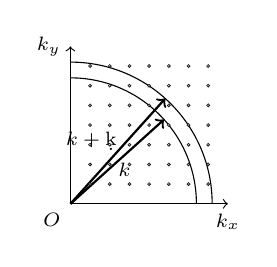
\begin{tikzpicture}[scale = .5, font = \scriptsize]
      \draw [<->] (0,4) node [left] {$k_y$} -- (0,0)
                        node [below left] {$O$} -- (4,0) node [below] {$k_x$};
      \draw (3.2,0) arc (0:90:3.2) (3.6,0) arc (0:90:3.6);
      \draw [thick, ->] (0,0) -- node [inner sep = 0pt, below right]
        {$k$} (42:3.2);
      \draw [thick, ->] (0,0) -- node [inner sep = 0pt, above left]
        {$k + \d k$} (48:3.6);
      \foreach \j in {1, ..., 7} \foreach \i in {1, ..., 7}
        \shade [shift = {(.5*\i, .5*\j)}, ball color = black]
          (0,0) circle (.05);
    \end{tikzpicture}
  \end{paracol}
  \begin{enumext}[label = (\alph*)]
    \item Determine the area in $k$-space occupied by one allowed $k$ point.
    \item Express number of allowed states in the area enclosed
    by the first quarter circles with the radus of $k$ and $k + \d k$,
    where $k \gg \d k$ (Consider the spin degeneracy).
    \item Express density of allowed states in real space per unit energy.
  \end{enumext}
\end{problem}
\begin{solution}\leavevmode
  \begin{enumext}[label = (\alph*)]
    \item The spaces of unit $k$ point
    in $k_x$-direction and $k_y$-direction are
    \[
      \Delta k_x = \frac\pi a, \qq{and} \Delta k_y = \frac\pi a
    \]
    Therefore, the area in $k$-space occupied by one allowed $k$ point is
    \[
      \Delta k_x \cdot \Delta k_y = \ab(\frac\pi a)^2
    \]
    \item The area enclosed by the two quarter circles is
    \[
      \d A = \frac14 2\pi k \d k = \frac{\pi k}{2} \d k
    \]
    Since every $k$ point occupy an area of $(\pi/a)^2$,
    so the number of allowed $k$-points in this area is
    \[
      \d N = \frac{2\d A}{(\pi/a)^2} = \frac{ka^2}{\pi} \d k
    \]
    Since two electrons can occupy each grid point
    ($\ket|\uparrow>$ and $\ket|\downarrow>$).
    \item Derivate it to the energy for a free election, we get
    \[
      \d E = \d\ab(\frac{\hbar^2 k^2}{2m}) = \frac{\hbar^2k}{m} \d k,
      \quad \d k = \frac{m \d E}{\hbar^2 k^2}.
    \]
    Substitute it into the result in (b): the number of states in $\d k$
    \[
      \d N = \frac{ka^2}{\pi} \d k = \frac{ma^2}{\pi\hbar^2} \d E,
    \]
    means in the whole system of area $a^2$,
    a number $\d N$ of states are allowed in energy range $\d E$.
    So, the density of allowed states in real space per unit energy is
    \[
      g(E) = \frac1{a^2} \odv NE = \frac{m}{\pi\hbar^2}.
    \]
  \end{enumext}
\end{solution}

\clearpage

\begin{problem}
  Density of states from a general formula:
  \begin{enumext}[label = (\alph*)]
    \item In a 3D solid and starting from the general formula,
    $g(E) = \frac{2V}{(2\pi)^3} \iint \frac{\d S_E}{\nabla_kE}$,
    find the expression for the electronic density of states:
    \begin{enumerate*}[label = (\roman*)]
      \item for free electrons;
      \item for electrons that obey the isotropic dispersion relation:
      $E = -E_0 - 2\gamma \cos\ab(\frac{ka}{2})$, where $E_0$, $\gamma > 0$.
    \end{enumerate*}
    \item After having established the corresponding expression for 2D,
    find $g(E)$ for (i) and (ii) above.
    \item Same question for 1D.
  \end{enumext}
\end{problem}
\begin{solution}
  Firstly, we shall calculate something before: For the isotropic dispersion
  \[
    E = -E_0 - 2\gamma \cos\ab(ka/2),
  \]
  we can obtain
  \[
    \sin\ab(\frac{ka}2) = \sqrt{1 - \ab(\frac{E+E_0}{2\gamma})^2}, \qq{and}
    k = \frac2a \arccos\ab(-\frac{E + E_0}{2\gamma}).
  \]
  Since $E = \hbar^2k^2/2m$, so $k = \sqrt{2mE/\hbar^2}$,
  $\nabla_k E = \hbar^2k/m$,
  $\nabla_k E = \gamma a \sin(ka/2)$ for isotropic dispersion.
  \begin{enumext}[label = (\alph*)]
    \item In a 3D situation, the general formula becomes
    \[
      g(E) = \frac{2V}{(2\pi)^3} \cdot \frac{4\pi k^2}{\hbar^2k/m}
    = \frac{Vmk}{\pi^2\hbar^2} = \frac{Vm}{\pi^2\hbar^3} \sqrt{2mE}.
    \]
    For isotropic dispersion, the general formula becomes
    \[
      g(E) = \frac{Vk^2}{\pi^2\gamma a\sqrt{1 - (\frac{E+E_0}{2\gamma})^2}}.
    \]
    \item In a 2D situation, the general formula becomes
    \[
      g(E) = \frac{2A}{(2\pi)^2} \cdot \frac{2\pi k}{\hbar^2k/m}
    = \frac{mA}{\pi\hbar^2} = \text{Const}.
    \]
    For isotropic dispersion, the general formula becomes
    \[
      g(E) = \frac{2A}{(2\pi)^2} \cdot \frac{2\pi k}{\gamma a \sin(ka/2)}
    = \frac{2A}{\pi\gamma a^2} \frac{\arccos\ab(-\frac{E+E_0}{2\gamma})}
        {\sqrt{1 - \ab(\frac{E+E_0}{2\gamma})^2}}
    \]
    \item In 1D situation, $g(E) = \frac{2L}{2\pi} \cdot \frac{2}{\odv E/k}$.
    The general formula becomes
    \[
      g(E) = \frac{2L}{2\pi} \cdot \frac{2}{\odv E/k} = \frac{2L}{\pi\odv E/k}
    = \frac L{\pi\hbar} \sqrt{\frac{2m}{E}}
    \]
    For isotropic dispersion, the general formula becomes
    \[
      g(E) = \frac{2L}{\pi\gamma a} \frac{1}{\sqrt{1 - \ab(\frac{E+E_0}{2\gamma})^2}}.
    \]
  \end{enumext}
\end{solution}